\subsubsection{La Contrôleur}
\label{subsubsec:controleur}

Afin de garantir le bon fonctionnement de notre application, nous avons implémenté un contrôleur qui permet de gérer les interactions entre les différentes parties de notre application. Le contrôleur est composé de plusieurs classes qui permettent de gérer les différents menus, les paramètres audio, les règles du jeu, la création de partie, la partie en elle-même, etc. C'est ce qui lie notre MVC et permet de faire fonctionner notre application.

\paragraph{Les mouvements}

% TODO: Parler des controleurs de mouvements

\paragraph{Les menus}

\paragraph{L'écran d'accueil}

Nous avons un écran d'accueil, géré par la classe StartMenu.java, qui possède des boutons pour:

\begin{itemize}
    \item Aller au menu de création de partie (Bouton Start)
    \item Aller au menu des paramètres audio (Bouton Engrenage)
    \item Afficher les règles du jeu (Bouton Start)
          %   \item Afficher les crédits
          % \item Quitter le jeu
\end{itemize}

Les différents éléments graphiques tels que le GIF et les images des boutons sont gérés par la classe JPanelWithImages.java.

\begin{figure}[h!]
    \centering
    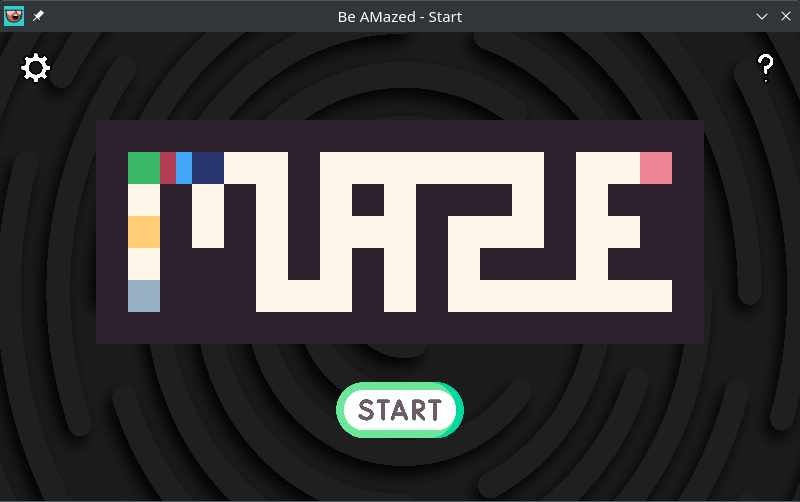
\includegraphics[scale=0.4]{ressources/Implementation/Labyrinthe/Controleur/StartMenu.png}%
    \caption{L'écran d'accueil}
    \label{fig:StartMenu}
\end{figure}